\documentclass[a4paper]{article}

\usepackage[UTF8]{ctex}
\usepackage[a4paper,margin=1in]{geometry}
\usepackage{graphicx}
\usepackage{float}
\usepackage{listings}
\usepackage{longtable}
\usepackage{booktabs}
\usepackage{hyperref}
\usepackage{fancyhdr}
\usepackage{lastpage}
\usepackage{color}
\usepackage{indentfirst}        % 首段缩进
\setlength{\parindent}{2em}     % 缩进2字符
\usepackage{zhnumber}           % 中文编号
\usepackage[dvipsnames]{xcolor}
\usepackage{array}              % 表格增强
\usepackage{tabularx}           % 自适应表格

\newcommand{\college}{中山大学计算机学院}
\newcommand{\projname}{软件工程课程项目}
\newcommand{\reporttitle}{LifeMaster软件开发文档}
\newcommand{\stuno}{项目团队}
\newcommand{\authorname}{刘昊、彭怡萱、马福泉、林炜东、刘贤彬、刘明宇}
\newcommand{\major}{软件工程}
\newcommand{\adviser}{郑贵锋}
\newcommand{\startdate}{2025年3月1日}
\newcommand{\labenddate}{2025年7月6日}
\newcommand{\labroom}{计算机学院}

\pagestyle{fancy} % 使用 fancyhdr 风格
\fancyhf{}      % 清空默认的页眉页脚

% 设置页眉
\fancyhead[L]{\kaishu \projname}      % 左侧页眉显示项目名称
\fancyhead[C]{\kaishu \reporttitle}    % 中间页眉显示报告标题
\fancyhead[R]{\kaishu 项目团队} % 右侧页眉显示项目团队

% 设置页脚
\fancyfoot[C]{第 \thepage 页,共 \pageref{LastPage} 页} % 中间页脚显示页码

% 去除页眉页脚与正文之间的分隔线
\renewcommand{\headrulewidth}{0.4pt}
\renewcommand{\footrulewidth}{0pt}


\begin{document}

% 封面
\begin{titlepage}
    \centering
    

    
\includegraphics[width=12cm]{img/SYSULogo.png}

    \vspace{1em}
    {\Large \college \par}
    \vspace{1em}
    {\Large \kaishu \projname \par}
    \vspace{3em}

    

      {\fontsize{40pt}{42pt}\kaishu \selectfont \boldmath \reporttitle\par}
    \vspace*{\fill}

    \begin{center}
    {\Large
    \makebox[5em][s]{项目名称}:\underline{\makebox[15em][c]{\kaishu LifeMaster}}\\[1em]
    \makebox[5em][s]{组员姓名}:\underline{\makebox[15em][c]{\kaishu 刘昊、彭怡萱、马福泉}}\\[0.5em]
    \makebox[5em][s]{}:\underline{\makebox[15em][c]{\kaishu 林炜东、刘贤彬、刘明宇}}\\[1em]
    \makebox[5em][s]{课程}:\underline{\makebox[15em][c]{\kaishu \major}}\\[1em]
    \makebox[5em][s]{课程教师}:\underline{\makebox[15em][c]{\kaishu \adviser}}\\[1em]
    \makebox[5em][s]{起始日期}:\underline{\makebox[15em][c]{\kaishu \startdate}}\\[1em]
    \makebox[5em][s]{结束日期}:\underline{\makebox[15em][c]{\kaishu \labenddate}}\\[1em]
    \makebox[5em][s]{学院}:\underline{\makebox[15em][c]{\kaishu \labroom}}
    }
    \end{center}

    \vspace*{\fill}
\end{titlepage}

% 目录
\tableofcontents
\newpage

\section{项目概述}

\subsection{产品背景}

在快节奏的现代生活中,人们面临着学习、工作、生活多方面的事务管理需求,同时也渴望通过便捷的方式记录生活点滴、进行自我提升与社交分享。LifeMaster 旨在打造一款集手账记录、任务管理、财务管理、小组协作及社区分享等功能于一体的综合性应用,帮助用户高效规划生活、学习和工作,满足其多样化的需求。

\subsection{产品目标}

\begin{itemize}
    \item 为用户提供便捷、高效的生活管理工具,提升用户在事务规划、时间管理和财务管理等方面的能力。
    \item 打造一个用户之间可以分享生活经验、学习资源的社交平台,增强用户之间的互动与交流。
    \item 成为用户日常生活中不可或缺的应用,提高用户使用频率和粘性,在同类产品中占据一定的市场份额。
\end{itemize}

\section{需求分析阶段}

\subsection{用户分析}

\subsubsection{目标用户群体}

\begin{itemize}
    \item \textbf{学生群体}:需要记录学习笔记、错题整理,与学习小组共享资料,同时希望通过记录生活手账来丰富课余生活。
    \item \textbf{职场人士}:面临工作任务繁多、时间紧张的问题,需要高效的任务管理和时间规划工具,也有记录工作心得和生活收支的需求。
    \item \textbf{自由职业者}:注重个人时间管理和财务管理,希望通过应用记录工作和生活的点滴,与同行进行交流分享。
    \item \textbf{生活爱好者}:喜欢记录生活中的美好瞬间,通过手账和社区分享功能展示自己的生活,与其他用户互动交流。
\end{itemize}

\subsubsection{用户痛点}

\begin{itemize}
    \item 缺乏一个能够整合多种生活管理功能的应用,导致用户需要使用多个不同的应用,操作繁琐。
    \item 学习和工作资料分散,难以进行统一管理和共享,影响效率。
    \item 现有的生活记录和社交分享应用功能单一,无法满足用户多样化的需求。
\end{itemize}

\subsection{功能需求}

\subsubsection{核心功能}

\paragraph{手账功能}

\begin{itemize}
    \item \textbf{内容记录}
    \begin{itemize}
        \item 文字编辑:支持丰富的文字格式设置,包括字体、字号、颜色、加粗、倾斜、下划线、段落排版等,方便用户撰写详细的日记、学习笔记或工作心得。
        \item 图片添加:用户可从相册、本地文件中选择图片插入手账,也支持拍照即时添加。插入的图片可进行缩放、裁剪、旋转、添加滤镜等操作,并能为图片添加说明。
        \item 贴纸装饰:系统提供精美贴纸,涵盖多种风格,用户可自由选择、拖动、调整大小和旋转角度,为手账增添趣味性和个性化元素。
    \end{itemize}
    \item \textbf{学习资料管理}
    \begin{itemize}
        \item 题目与错题记录:用户可在手账中添加题目和错题,支持图片、文字等多种格式。对于错题,可详细记录错误原因、正确解法和相关知识点,方便复习巩固。
        \item 资料分类整理:提供文件夹分类和标签功能,用户可创建不同的分类文件夹,如"数学错题集""语文作文素材"等,并为每篇手账添加多个标签,如"函数知识点""议论文写作技巧",实现快速检索。
    \end{itemize}
    \item \textbf{分享与协作}
    \begin{itemize}
        \item 个人回顾与小组共享:手账默认仅自己可见,用户可一键将手账设置为小组共享,小组成员可在线查看、评论、点赞共享的手账内容,实现学习资源的高效共享与交流。
        \item 社区分享:用户可将优质手账分享至社区,其他用户可在社区浏览、点赞、评论、转发,形成良好的互动氛围。
    \end{itemize}
\end{itemize}

\paragraph{任务管理功能}

\begin{itemize}
    \item 任务创建与编辑:用户可创建新任务,输入任务标题、详细描述、截止时间、优先级等信息,并可随时对任务进行编辑修改。
    \item 任务分类与排序:支持按照任务类型(如工作、学习、生活)、优先级(高、中、低)、截止时间等进行分类和排序,方便用户快速查找和管理任务。
    \item 任务状态管理:任务状态包括待办、进行中、已完成,用户可通过简单操作切换任务状态,直观展示任务进度。
    \item 任务提醒:用户可设置任务提醒时间,提醒方式包括消息通知、铃声提醒等。
    \item 任务统计与分析:系统自动统计任务完成情况,生成任务完成率、逾期任务数量等数据报表,并以图表形式展示,帮助用户分析任务管理效率。
\end{itemize}

\paragraph{财务管理功能}

\begin{itemize}
    \item 收支记录:用户可记录每一笔收入和支出,包括金额、时间、分类(如餐饮、购物、工资、奖金等)、备注等信息,支持快速输入和批量导入。
    \item 收支分类管理:用户可自定义收支分类,设置分类图标和名称,方便对收支情况进行分类统计和分析。
    \item 收支统计与报表:系统自动生成收支明细列表、月度收支汇总表、收支占比饼状图等,直观展示用户的财务状况,帮助用户分析消费习惯,制定合理的理财计划。
    \item 预算管理:用户可设置月度、年度预算,系统实时显示预算使用情况,当接近或超过预算时,发出预警提醒。
\end{itemize}

\subsubsection{扩展功能}

\paragraph{小组共享功能}

\begin{itemize}
    \item 小组创建与管理:用户可创建新小组,设置小组名称、简介、成员邀请方式等信息。小组创建者可管理小组成员,包括添加、删除成员,设置成员权限(如查看、编辑、评论等)。
    \item 共享内容管理:小组成员可上传共享手账、学习资料、任务列表等内容,支持对共享内容进行分类管理和版本控制。
    \item 小组讨论与交流:小组内提供聊天功能,成员可针对共享内容进行讨论交流,提高小组协作效率。
\end{itemize}

\paragraph{番茄钟功能}

\begin{itemize}
    \item 专注时间设置:用户可自定义专注时长和休息时长,支持常见的时间设置(如25分钟专注+5分钟休息),也可根据个人需求进行个性化设置。
    \item 倒计时与提醒:在专注和休息过程中,系统显示倒计时,倒计时结束后发出消息通知和铃声提醒,帮助用户合理安排时间,提高工作和学习效率。
    \item 番茄钟记录与统计:系统自动记录用户每次使用番茄钟的时间、次数等数据,生成统计报表,用户可查看自己的时间使用情况,分析时间管理效果。
\end{itemize}

\paragraph{社区分享功能}

\begin{itemize}
    \item 内容发布:用户可在社区发布手账、学习经验、生活技巧、资源链接等内容,支持图文混排、视频上传等多种形式。
    \item 内容浏览与搜索:社区提供按分类浏览、热门推荐、最新发布等多种浏览方式,用户也可通过关键词搜索感兴趣的内容。
    \item 互动交流:用户可对感兴趣的内容进行点赞、评论、转发,关注其他用户,建立社交关系,形成良好的社区氛围。
\end{itemize}

\subsection{非功能需求}

\subsubsection{性能需求}

\begin{itemize}
    \item 响应时间:在正常网络环境下,页面加载时间不超过3秒,数据查询响应时间不超过1秒,操作交互响应及时,无明显卡顿。
    \item 并发处理能力:系统能够支持至少1000用户同时在线,保证在高并发情况下,核心功能(如任务创建、手账记录)的响应时间和稳定性不受明显影响。
    \item 数据处理能力:能够快速处理大量的用户数据,包括手账记录、任务信息、财务数据等,确保数据的存储、查询和统计效率。
\end{itemize}

\subsubsection{安全性需求}

\begin{itemize}
    \item 数据安全:对用户的敏感数据(如登录密码、财务信息)进行加密存储,采用SSL/TLS加密协议保障数据在传输过程中的安全性,防止数据泄露和篡改。
    \item 系统安全:定期进行系统安全漏洞扫描和修复,防范网络攻击(如SQL注入、XSS攻击),确保系统的稳定性和安全性。
\end{itemize}

\subsubsection{兼容性需求}

\begin{itemize}
    \item 设备兼容性:支持在各种主流操作系统(Linux、Windows)正常运行,保证界面显示正常、功能操作流畅。
    \item 浏览器兼容性:提供Web端访问,确保在主流浏览器(Chrome、Firefox、Safari、Edge)上能够正常显示和使用,兼容不同版本的浏览器。
\end{itemize}

\subsubsection{易用性需求}

\begin{itemize}
    \item 界面设计:采用简洁、美观、直观的界面设计风格,符合用户的使用习惯和审美需求。界面布局合理,功能入口清晰,操作流程简单易懂。
    \item 操作便捷性:提供便捷的操作方式,如快捷按钮、批量操作等,减少用户的操作步骤和时间成本。对重要操作进行二次确认提示,防止用户误操作。
\end{itemize}

\section{设计阶段}

\subsection{系统设计文档}

\subsubsection{架构图}

\textbf{架构类型:}前端-后端-数据库三层架构

\textbf{架构图说明:}

\begin{figure}[H]
\centering
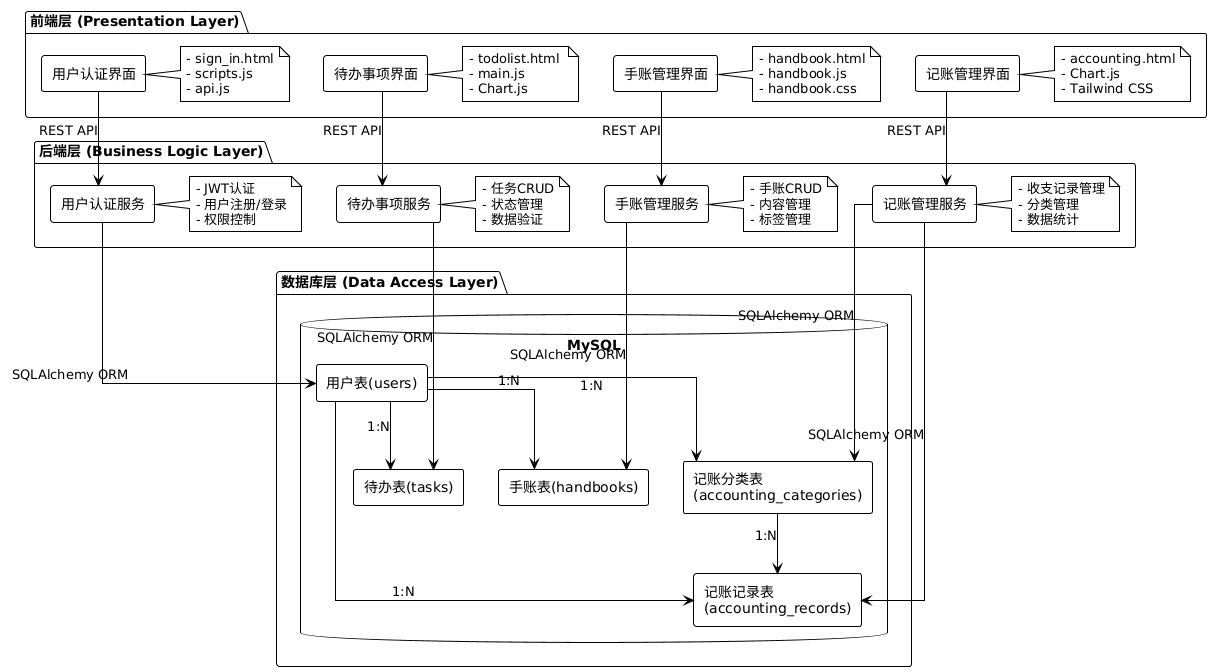
\includegraphics[width=1.0\textwidth]{img/architecture.png}
\caption{LifeMaster系统架构图}
\end{figure}

\begin{itemize}
    \item 前端层:负责用户界面渲染与交互(表示层)
    \item 后端层:处理业务逻辑与接口响应(业务逻辑层)
    \item 数据层:数据库存储与数据管理(数据访问层)
\end{itemize}

\subsubsection{技术选型}

\begin{table}[H]
\centering
\begin{tabular}{|l|l|l|}
\hline
\textbf{模块} & \textbf{技术/工具} & \textbf{说明} \\
\hline
前端框架 & HTML5+CSS3+JavaScript & 原生前端技术,支持响应式设计 \\
\hline
后端框架 & Flask & 轻量级Python Web框架 \\
\hline
数据库 & MySQL 5.7+ & 关系型数据库,支持事务与索引 \\
\hline
版本控制 & Git+GitHub & 团队协作与代码管理 \\
\hline
\end{tabular}
\caption{技术选型表}
\end{table}

\subsection{详细设计文档}

\subsubsection{类图(UML)}

\textbf{核心类说明:}

\begin{figure}[H]
\centering
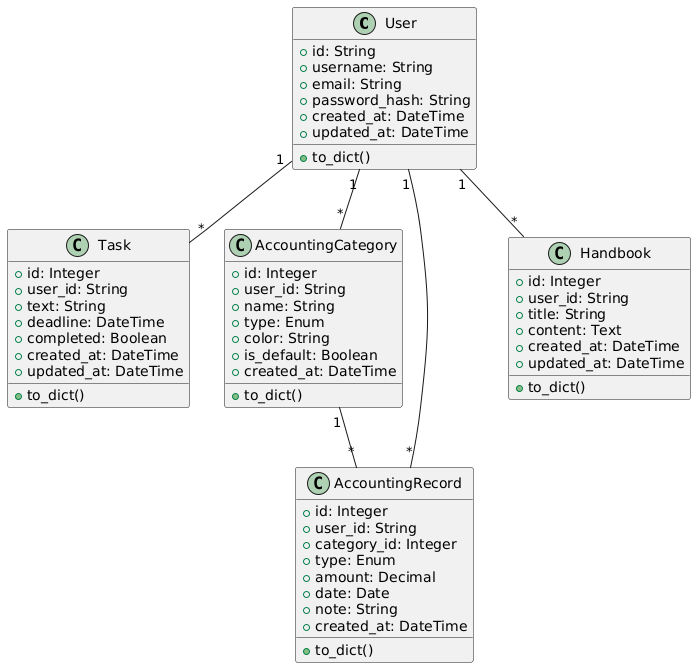
\includegraphics[width=0.8\textwidth]{img/class_diagram.png}
\caption{LifeMaster核心类图}
\end{figure}

\begin{itemize}
    \item User类:用户基本信息(ID、用户名、权限等)
    \item Handbook类:手账记录(标题、内容、创建时间等)
    \item Task类:任务管理(标题、截止时间、状态等)
\end{itemize}

\subsubsection{顺序图(UML)}

\begin{figure}[H]
\centering
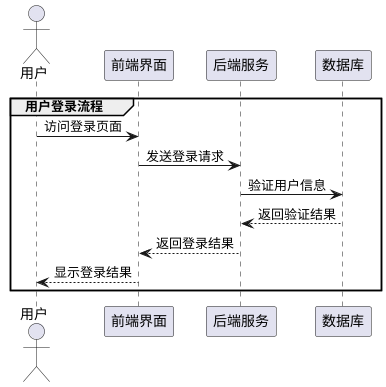
\includegraphics[width=0.6\textwidth]{img/sequence_diagram1.png}
\caption{LifeMaster用户登录流程顺序图}
\end{figure}

\begin{figure}[H]
\centering
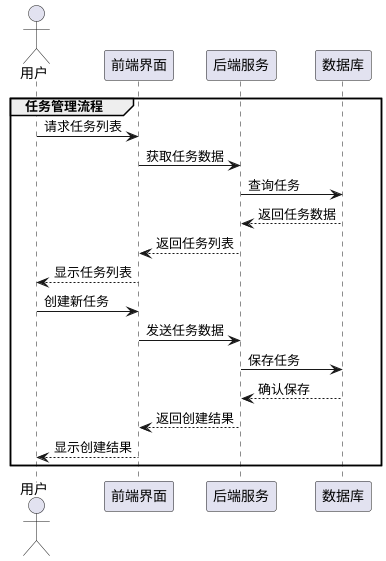
\includegraphics[width=0.8\textwidth]{img/sequence_diagram2.png}
\caption{LifeMaster财务管理流程顺序图}
\end{figure}

\begin{figure}[H]
\centering
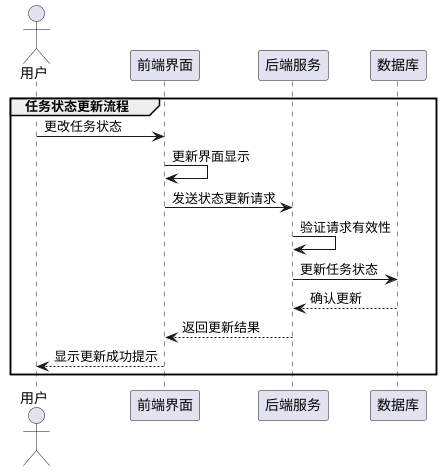
\includegraphics[width=0.8\textwidth]{img/sequence_diagram3.png}
\caption{LifeMaster手账管理流程顺序图}
\end{figure}

\begin{figure}[H]
\centering
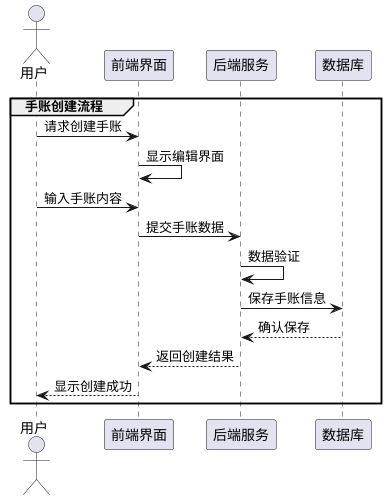
\includegraphics[width=0.8\textwidth]{img/sequence_diagram4.png}
\caption{LifeMaster任务管理流程顺序图}
\end{figure}

\textbf{顺序图示例场景:}

\paragraph{用户登录流程}
用户访问登录页面→前端发送登录请求到后端→后端查询数据库验证用户信息→数据库返回验证结果→后端生成token返回前端→前端显示登录结果并跳转

\paragraph{财务管理流程}
\begin{itemize}
    \item 记财分类管理:用户点击``分类管理''按钮→前端请求分类列表数据→后端从数据库查询分类→数据库返回分类数据→后端处理并返回前端→前端渲染分类列表
    \item 记账记录管理:用户填写收支记录表单→前端进行表单数据验证→前端提交记录数据到后端→后端处理业务逻辑→后端将数据存入数据库→数据库确认存储完成→返回操作结果给用户
    \item 账务统计分析:用户查看财务报表→前端请求统计数据→后端执行数据库聚合查询→数据库返回统计结果→后端处理数据返回前端→前端生成可视化图表→向用户展示财务报表
\end{itemize}

\paragraph{手账创建流程}
用户点击``新建手账''按钮→前端显示手账编辑界面→用户输入手账标题和内容→前端提交手账数据到后端→后端验证数据完整性→后端将手账保存到数据库→数据库确认保存成功→前端显示创建成功提示

\paragraph{任务状态更新}
用户点击任务状态切换按钮→前端立即更新界面显示→前端发送状态更新请求→后端验证请求合法性→后端更新数据库中的任务状态→数据库确认更新完成→返回更新结果到前端→前端显示更新成功提示

\subsubsection{用例图(UML)}

\begin{figure}[H]
\centering
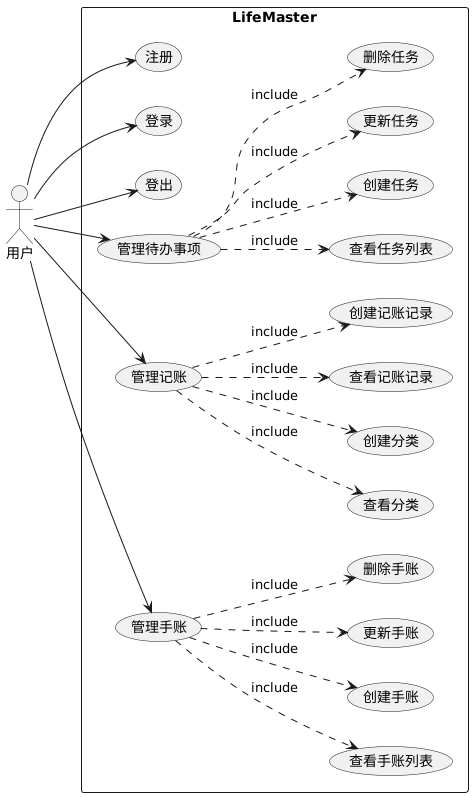
\includegraphics[width=0.8\textwidth]{img/use_case_diagram.png}
\caption{LifeMaster用例图}
\end{figure}

\subsubsection{活动图(UML)}

\begin{figure}[H]
\centering
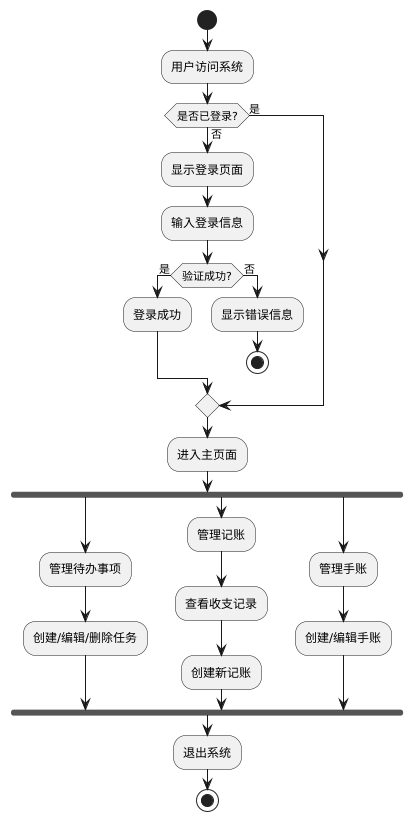
\includegraphics[width=0.6\textwidth]{img/activity_diagram.png}
\caption{LifeMaster活动图}
\end{figure}

\subsubsection{状态图(UML)}

\begin{figure}[H]
\centering
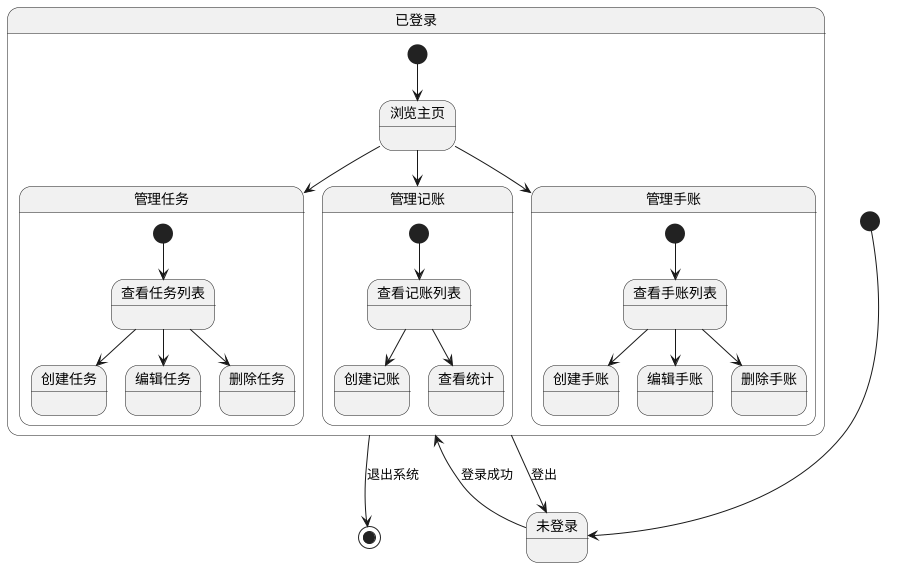
\includegraphics[width=0.8\textwidth]{img/state_diagram.png}
\caption{LifeMaster状态图}
\end{figure}

\subsection{数据库设计}

% 这里会从database.md中添加数据库设计内容

\subsection{接口设计(API文档)}

API文档详见:\url{https://kdocs.cn/l/ce088HbETBdM}

\section{开发阶段}

\subsection{人员分工}

\begin{table}[H]
\centering
\begin{tabular}{|l|l|l|}
\hline
\textbf{任务项} & \textbf{负责人} & \textbf{完成标志} \\
\hline
前端页面开发 & 彭怡萱、刘昊 & 页面交互demo验收 \\
\hline
后端接口开发 & 刘贤彬、刘明宇 & 接口文档与自测报告 \\
\hline
数据库设计 & 马福泉、林炜东 & 数据库设计文档 \\
\hline
\end{tabular}
\caption{人员分工表}
\end{table}

\subsection{开发者指南}

\subsubsection{环境配置}

\begin{itemize}
    \item Python 3.8+,Flask 2.0+,MySQL 5.7+
    \item 前端依赖:Tailwind CSS
\end{itemize}

\subsubsection{构建步骤}

\begin{itemize}
    \item 克隆代码库:\url{https://github.com/cornhub919/LIFEmaster.git}
    \item 后端:按照环境配置要求搭建Python+Flask环境
    \item 前端:直接打开HTML文件
\end{itemize}

\subsubsection{前端实现}

\begin{itemize}
    \item 使用``即时设计'',绘制UI界面样式
    \item HTML结构语义化
    \item CSS类名使用Tailwind规范
    \item JavaScript函数按功能封装
\end{itemize}

% 这里可以添加前端界面截图
% \begin{figure}[H]
% \centering
% \includegraphics[width=0.8\textwidth]{img/frontend_ui.png}
% \caption{前端界面设计}
% \end{figure}

\subsubsection{后端实现}

\begin{itemize}
    \item 基于Flask实现
    \item 提供函数接口,基于函数接口实现功能
\end{itemize}

\subsubsection{数据库实现}

\paragraph{环境准备}

\textbf{1. 安装依赖}

\begin{lstlisting}[language=bash]
pip install flask flask-sqlalchemy flask-jwt-extended flask-cors pymysql python-dotenv
\end{lstlisting}

\textbf{2. 环境配置}

创建 .env 文件:
\begin{lstlisting}[basicstyle=\ttfamily]
DB_HOST=localhost
DB_PORT=3306
DB_USER=root
DB_PASSWORD=???
DB_NAME=lifemaster
JWT_SECRET_KEY=your-secret-key-123
\end{lstlisting}

\paragraph{MySQL数据库设置}

\textbf{1. 启动MySQL服务}

\begin{lstlisting}[language=bash]
Windows
net start mysql
mysql --version
\end{lstlisting}

\textbf{2. 创建数据库}

\begin{lstlisting}[language=sql]
mysql -u root -p
CREATE DATABASE lifemaster CHARACTER SET utf8mb4 COLLATE utf8mb4_unicode_ci;
SHOW DATABASES;
exit;
\end{lstlisting}

\textbf{3. 测试连接}

\begin{lstlisting}[language=python]
python -c "
import pymysql;
import os;
from dotenv import load_dotenv;
load_dotenv();
try:
    conn = pymysql.connect(host='localhost', user='root', 
                          password=os.getenv('DB_PASSWORD'), 
                          database='lifemaster');
    print('Database connection successful!');
    conn.close()
except Exception as e:
    print(f'Connection failed: \{e\}')
"
\end{lstlisting}

\paragraph{Flask数据库初始化}

\textbf{1. 初始化数据库迁移}

\begin{lstlisting}[language=bash]
flask db init

flask db migrate -m "Initial migration"

flask db upgrade
\end{lstlisting}

\textbf{2. 创建数据表}

\begin{lstlisting}[language=python]
python -c "from app import app, db; app.app_context().push(); 
           db.create_all(); print('Tables created successfully!')"
\end{lstlisting}

\textbf{3. 创建管理员用户(可选)}

\begin{lstlisting}[language=python,basicstyle=\ttfamily,breaklines=true]
python -c "
from app import app, db, User, AccountingCategory;
from werkzeug.security import generate_password_hash;
app.app_context().push();
user = User(username='admin', email='admin@lifemaster.com', 
           password_hash=generate_password_hash('admin123'));
db.session.add(user);
db.session.commit();
print('Admin user created! username:admin password:admin123')
"
\end{lstlisting}

\paragraph{启动应用}

\textbf{1. 启动后端}

\begin{lstlisting}[language=bash]
python app.py
\end{lstlisting}

访问:\url{http://localhost:5000}

\textbf{2. 启动前端}

\begin{lstlisting}[language=bash]
cd frontend
python -m http.server 8080
\end{lstlisting}

访问:\url{http://localhost:8080/sign_in.html}

\textbf{3. 一键启动(推荐)}

\begin{lstlisting}[language=bash]
# Generate standalone executable file
\end{lstlisting}

\section{测试阶段}

\subsection{测试计划(敏捷迭代测试)}

\subsubsection{测试范围}

\begin{itemize}
    \item 单元测试:后端接口函数、数据处理逻辑
    \item 集成测试:前后端数据交互、模块间协作
    \item 系统测试:完整功能流程(如手账创建-共享-查看)
\end{itemize}

\subsubsection{测试策略}

\begin{itemize}
    \item 每个迭代周期(一次会议为一个迭代周期)完成后进行冒烟测试
    \item 核心功能(手账、任务、记账)采用100\%测试用例覆盖
\end{itemize}

\subsection{测试文档报告}

\begin{table}[H]
\centering
\begin{tabular}{|l|l|l|l|l|l|}
\hline
\textbf{模块} & \textbf{用例名称} & \textbf{输入数据} & \textbf{预期输出} & \textbf{实际结果} & \textbf{状态} \\
\hline
任务管理 & 添加待办任务 & 任务标题"开会",截止时间明天 & 任务列表显示"开会",状态为"进行中" & 正常显示 & 通过 \\
\hline
财务管理 & 记录支出 & 类型"支出",金额100,分类"餐饮" & 本月支出增加100,饼状图更新 & 数据正确 & 通过 \\
\hline
手账共享 & 小组内修改共享手账 & 加入小组后修改他人共享手账 & 修改后小组成员可查看最新版本 & 同步更新 & 通过 \\
\hline
\end{tabular}
\caption{测试报告示例}
\end{table}

\subsection{测试验证}

\subsubsection{登录测试}

\begin{itemize}
    \item 用户名:admin
    \item 邮箱:admin@lifemaster.com
    \item 密码:admin123
\end{itemize}

\subsubsection{API测试}

\begin{lstlisting}[language=bash]
# test login API
curl -X POST http://localhost:5000/api/auth/login \
  -H "Content-Type: application/json" \
  -d '\{"email":"admin@lifemaster.com","password":"admin123"\}'
\end{lstlisting}

\subsubsection{用户数据隔离测试}

\begin{lstlisting}[language=bash]
# Test user isolation
python test/test_user_isolation.py
\end{lstlisting}

\textbf{测试内容:}
\begin{itemize}
    \item 不同用户的待办事项独立
    \item 不同用户的记账记录独立
    \item 不同用户的手账独立
    \item 用户只能看到自己的数据
\end{itemize}

\section{部署与维护阶段}

\subsection{部署流程}

\begin{enumerate}
    \item 配置生产环境数据库
    \item 部署后端服务
    \item 配置前端静态资源
    \item 配置反向代理和负载均衡
    \item 配置监控和日志系统
\end{enumerate}

\subsection{维护策略}

\begin{itemize}
    \item 定期数据库备份
    \item 系统性能监控
    \item 安全漏洞扫描
    \item 用户反馈收集与处理
\end{itemize}

\subsection{常见问题解决}

\subsubsection{问题1:数据库连接失败}

解决方案:
\begin{enumerate}
    \item 检查MySQL服务:net start mysql
    \item 验证密码:mysql -u root -p
    \item 检查.env配置
\end{enumerate}

\subsubsection{问题2:模块导入失败}

解决方案:
\begin{lstlisting}[language=bash]
pip install flask flask-sqlalchemy pymysql
\end{lstlisting}

\subsubsection{问题3:数据库重置}

\begin{lstlisting}[language=python]
# Reset database (will delete all data)
python -c "from app import app, db; app.app_context().push(); 
           db.drop_all(); db.create_all(); print('Database reset complete!')"
\end{lstlisting}

\section{项目总结}

\subsection{项目成果}

在本次LifeMaster软件开发项目中,我们团队成功完成了以下工作:

\begin{enumerate}
    \item 完成了需求分析,明确了目标用户群体和功能需求
    \item 设计了完整的系统架构和数据库结构
    \item 实现了手账记录、任务管理、财务管理等核心功能
    \item 构建了前后端分离的Web应用架构
    \item 完成了系统测试和部署工作
\end{enumerate}

\subsection{技术收获}

通过本项目的开发,团队成员在以下方面获得了技术提升:

\begin{itemize}
    \item 掌握了Flask Web框架的使用
    \item 学习了前后端分离的开发模式
    \item 熟悉了MySQL数据库的设计和操作
    \item 体验了敏捷开发和团队协作
\end{itemize}

\subsection{项目改进建议}

\begin{enumerate}
    \item 增加移动端适配,提升用户体验
    \item 优化数据库性能,支持更大用户量
    \item 完善安全机制,加强数据保护
    \item 增加更多社交功能,提升用户粘性
\end{enumerate}

\section{附录参考资料}
\begin{thebibliography}{99}  

    \bibitem{ref1}LifeMaster项目团队. (2025). LifeMaster软件开发项目. GitHub. \url{https://github.com/cornhub919/LIFEmaster.git}
    \bibitem{ref2}金蝶云. (2025). API接口文档. 金蝶文档. \url{https://kdocs.cn/l/ce088HbETBdM}
    \bibitem{ref3}Flask官方文档. (2025). Flask Web开发框架. Website. \url{https://flask.palletsprojects.com/}
    \bibitem{ref4}MySQL官方文档. (2025). MySQL数据库管理系统. Website. \url{https://dev.mysql.com/doc/}
    \bibitem{ref5}Tailwind CSS官方文档. (2025). Tailwind CSS框架. Website. \url{https://tailwindcss.com/docs}

\end{thebibliography}

\section{附录代码清单}

本项目的完整代码包括前端HTML/CSS/JavaScript文件和后端Python Flask代码,详细代码请参见项目GitHub仓库:

\url{https://github.com/cornhub919/LIFEmaster.git}

主要文件结构:
\begin{itemize}
    \item \texttt{app.py} - Flask主应用文件
    \item \texttt{前端/} - 前端页面文件夹
    \item \texttt{.env} - 环境配置文件
    \item \texttt{database.md} - 数据库配置指南
    \item \texttt{生成exe.bat} - 打包脚本
\end{itemize}

\end{document}